%! Author = user
%! Date = 13.06.2023

\documentclass[a4paper, 14pt]{article}
%\documentclass[draft]{article}

\usepackage[T2A]{fontenc}
\usepackage[utf8]{inputenc}
\usepackage[english, russian]{babel}
\usepackage[top = 2cm, bottom = 2cm, left = 2cm, right = 2cm]{geometry}
\usepackage{indentfirst}
\usepackage{xcolor}
\usepackage{hyperref}
\usepackage{gensymb}
\usepackage{pgfplots}
\usepackage{amsmath, amsfonts, amsthm, mathtools}
\usepackage{amssymb}
\usepackage{physics, multirow, float}
\usepackage{wrapfig, tabularx}
\usepackage{icomma} % Clever comma: 0,2 - number while 0, 2 - two numbers
\usepackage{tikz, standalone}
\usepackage{fancyhdr,fancybox}
\usepackage{lastpage}
\usepackage{booktabs}
\usepackage{listings}
\usepackage{lstmisc}
\usepackage{stmaryrd}
\usepackage{amstex}

%\полуторный интервал
\onehalfspacing

\hypersetup
{   colorlinks = false,
    linkcolor = blue,
    pdftitle = {genphys},
    pdfauthor = {Володин Максим},
    allcolors = [RGB]{010 090 200}
}

\graphicspath{{./images/}}
\DeclareGraphicsExtensions{.pdf,.png,.jpg}

\restylefloat{table}
\usetikzlibrary{external}

\mathtoolsset{showonlyrefs = true} % Numbers will appear only where \eqref{} in the text LINKED
\pagestyle{fancy}

\fancyhf{}
\fancyhead[L]{Вопрос по выбору}
\fancyhead[R]{Гидравлический удар}
\fancyfoot[L]{}
\fancyfoot[R]{\thepage /\pageref{LastPage}}

\pgfplotsset{compat=1.18}

\begin{document}
    \begin{titlepage}
        \begin{center}
        {\large МОСКОВСКИЙ ФИЗИКО-ТЕХНИЧЕСКИЙ ИНСТИТУТ \\ \vspace{5mm}
        НАЦИОНАЛЬНЫЙ ИССЛЕДОВАТЕЛЬСКИЙ УНИВЕРСИТЕТ \\ \vspace{5mm}
        КАФЕДРА ОБЩЕЙ ФИЗИКИ}
        \end{center}

        \begin{center}
        {\large}
        \end{center}

        \vspace{5cm}

        {\huge
            \begin{center}
                \textbf{Вопрос по выбору}
                \\ Гидравлический удар
            \end{center}
        }

        \vspace{2cm}

        \begin{flushright}
        {
            Володин Максим \\
            \vspace{2mm}
            Б02-206 \\
            \vspace{2mm}
            Физтех-школа физики и исследований имени Ландау
        }
        \end{flushright}

        \tableofcontents \vspace{6cm}

        \begin{center}
            Долгопрудный \\
            14 января 2023 года
        \end{center}

    \end{titlepage}


    \section{Фазы удара}

    Гидравлический удар -- скачок давления в какой-либо системе, заполненной жидкостью, вызванный быстрым изменением
    скорости (остановкой) потока этой жидкости.
    В случае большой скорости и неупругости материала труб происходит пробой последних

    Рассмотрим возникновение гидроудара на самом простом примере -- внезапном заполнении жидкостью пустой трубы
    постоянного сечения, погружённой на некоторую глубину $H$ и глубиной избыточного погружения $h$.
    Один конец этой трубы запаян, а другой свободно сообщается с окружающей жидкостью (можно рассматривать и
    аналогичные примеры: падение пробирки, опускание заслонки \ldots). Голубым цветом обозначена внешняя среда с
    исходным давлением, светло-голубым — область пониженного давления, синим — область повышенного давления (зона
    гидроудара).
    Синие стрелки показывают перемещение вещества среды (жидкости), красные — перемещение границы зоны повышенного
    давления (без существенного перемещения вещества.
    Процесс состоит из семи этапов:

    \begin{figure}
        \begin{center}
            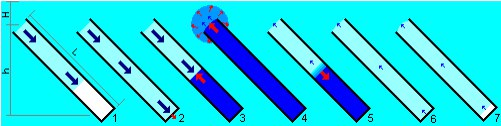
\includegraphics[width=0.8\textwidth]{phases}
        \end{center}
        \caption{Схема возникновения гидравлического удара при заполнении жидкостью пустой трубы~\cite{3}}
%    \label{phases}
    \end{figure}

    \begin{enumerate}
        \item \textit{Заполнение трубы жидкостью (уравнение Бернулли)}

        \item \textit{Встреча с препятствием}.
        Жёсткая заглушка внезапно останавливает поток, который ударяется в неё.
        Однако практически вся жидкость в трубе ещё продолжает своё движение вперёд

        \item \textit{Рост зоны повышенного давления}.
        Головная часть потока остановилась и её кинетическая энергия перешла в потенциальную энергию упругой
        деформации жидкости и \uline{стенок} трубы, вызвав в этой области повышение давление.
        В силу конечности скорости распространения ($\approx c$) деформации до «хвоста» потока это воздействие ещё не
        дошло

        \item \textit{Максимум повышенного давления}.
        Ударная волна достигла входа трубы и вышла в неподвижную среду.
        Таким образом, достигнув входа трубы, ударная волна «рассеивается» и «гаснет»

        \item \textit{Начало обратного движения}.
        Поскольку у входа в трубу давление относительно невысоко, сжатая жидкость двигается туда под действием
        повышенного давления внутри трубы.
        При этом потенциальная энергия упругой деформации снова превращается в кинетическую энергию, но движение уже
        направлено в обратную сторону.
        В результате граница зоны неподвижной жидкости под повышенным давлением перемещается (со скоростью порядка $c$)
        от входа в трубу обратно к заглушке, оставляя у входа зону немного пониженного давления, в которой жидкость
        движется обратно ко входу трубы

        \item \textit{Окончание сжатия}.
        В момент, когда граница зоны пониженного давления достигает заглушки, во всей трубе жидкость снова испытывает
        пониженное давление и движется обратно ко входу со скоростью, равной скорости потока в трубе в фазе 2

        \item \textit{Фаза разрежения (отрыва)}.
        Двигаясь в сторону входа трубы, жидкость в силу инерции стремится оторваться от заглушки.
        Поэтому, если гидроудар был достаточно сильным, то возле заглушки образуется зона разрежения, где жидкость
        отсутствует и давление близко к нулю (именно к вакууму, если удар достаточно силён).
        Однако жидкость, выходящая из трубы, движется не в пустоту, а в среду, представляющую собой ту же жидкость,
        только неподвижную.
        Сопротивление этой среды достаточно быстро затормозит движение жидкости к выходу и вместе с зоной разрежения
        возле заглушки вновь заставит жидкость двигаться от входа внутрь трубы, тем самым повторяя фазу 1.
        Начинаются затухающие колебания

    \end{enumerate}


    \section{Условие отрыва жидкости}

    Как говорилось раннее, в фазе разрежения отрыв жидкости от заглушки происходит не всегда.
    Для того чтобы жидкость смогла оторваться от заглушки и появилась область отрыва, обратное давление (в идеале,
    без учёта потерь, равное максимальному повышению давления при сжатии) должно превышать давление среды снаружи.
    Таким образом, отрыв жидкости с образованием вакуума возможен при выполнении условия $\Delta P_{\text{уд}} > P_0
    + h \Delta P + Q $, где $\Delta P_{\text{уд}}$ --- максимальное повышение давления в фазе сжатия относительно
    внешнего давления, $P_0$ --- абсолютное внешнее давление в резервуаре возле входа в трубу (т.е. давление
    относительно вакуума, а не атмосферы над поверхностью жидкости); $h \Delta P$ --- гидростатическая разность
    давлений между входом в трубу и заглушкой, если труба расположена не горизонтально; $Q$ --- необратимые потери
    давления при сжатии и расширении жидкости и стенок трубы в фазах 2--6

    Если пренебречь потерями, то для строго горизонтальной трубы критерий возникновения области вакуума будет ещё
    проще: $\Delta P_{\text{уд}} > P_0$.
    Может возникнуть вопрос: как же повышение давления при гидроударе может превысить давление на входе в трубу?
    Однако здесь нет парадокса, так как скачок давления зависит лишь от резкости остановки потока и набранной им к
    этому моменту кинетической энергии, поэтому жёсткая труба и несжимаемая жидкость могут обеспечить сильный удар
    даже при не слишком высокой скорости потока.
    Таким образом, удары можно разделить на слабо- и сильномощные (из-за резкости, а не энергии)


    \section{Анализ возникающих колебаний}

    \begin{figure} [h]
        \begin{center}
            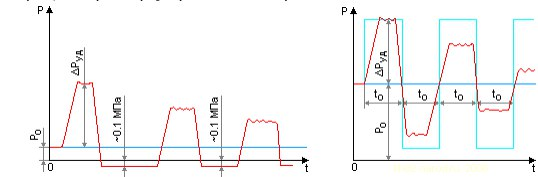
\includegraphics[width=0.8\textwidth]{flucts}
        \end{center}
        \caption{График зависимости $P(t)$ для давления у заглушки~\cite{3}}
%    \label{fig:flucts}
    \end{figure}

    Посмотрим, как при гидроударе с течением времени изменяется давление возле заглушки.
    На рисунке видно, что при сильном гидроударе (слева) в фазе отрыва давление падает практически до нуля, т.е.
    образуется вакуум (0,1 МПа $=$ 1 атм, давление измерялось относительно атмосферного, поэтому показания в –1 атм
    как раз и соответствуют абсолютному нулю давления).
    Однако это не слишком снижает энергию повторных гидроударов, более того, характер их постепенного ослабления не
    отличается от аналогичного ослабления при слабом гидроударе, показанном на рисунке справа

    При слабом гидроударе (без отрыва жидкости), фазы сжатия и разрежения имеют одинаковую длительность $t_0$,
    обусловленную временем «путешествия» ударной волны от заглушки ко входу трубы и обратно.
    В этом случае возмущения не выходят в резервуар сколько-нибудь далеко от входа трубы, и период этих колебаний
    полностью определяется длиной трубы и скоростью ударной волны

    Повторный удар получается сильным, однако «затишье» между ударами существенно больше длительности каждого удара,
    поскольку ударная волна выходит далеко за пределы трубы, и этот путь требует дополнительного времени.
    По мере снижения силы повторных ударов интервал между ними сокращается, и когда скачок давления при очередном
    повторном гидроударе $\Delta P_{\text{уд}}$ становится равным давлению вне трубы $P_0$, сравнивается с $t_0$ и в
    дальнейшем уже не уменьшается

    В каждом цикле гидроудара площади положительного и отрицательного отклонения от уровня давления $P_0$ графике $P(
    t)$ должны быть равны, поскольку они пропорциональны энергии, а без учёта потерь энергия стадии сжатия и стадии
    расширения должна быть одинаковой.


    \section{Расчёты}

    \noindent Условие соотношения длительностей стадий сжатия и разрежения возле заглушки в следующем виде:
    \[ (P_0 - P_{\text{сж}}) t_{\text{сж}} = (P_{\text{расш}} - P_0) t_{\text{расш}} \text{ или } \Delta P_{\text{сж}}
    t_{\text{сж}} = -\Delta P_{\text{расш}} t_{\text{расш}} \]
    Величину давления у задвижки легче всего получить исходя из закона сохранения импульса:
    \begin{gather*}
        \rho S v dl = \Delta P S dt \text{, где } v \text{ -- скорость потока перед его установкой (Бернулли)}\\
        \Delta P = \rho v \frac{dl}{dt} = \rho v u \text{, где } u \text{ -- скорость звука в воде}\\
    \end{gather*}
    Величина ускорения потока жидкости:
    \begin{gather*}
        F = (\Delta P + \frac{\rho v^2}{2}) \pi R^2\\
        a = \frac{F}{m} = (\Delta P + \frac{\rho v^2}{2}) \frac{\pi R^2}{\pi R^2 x} = \frac{(\Delta P + \frac{\rho
        v^2}{2})}{x}\\
    \end{gather*}
    Время периода собственных колебаний ударной волны:
    \[ T = \frac{2L}{u} \]

    Эта величина достаточно мала.
    Скорость звука в жидкостях обычно составляет порядка 1000\dots1500 м/с (для воды при 4°С — 1,44 км/с, при 45°С 1,51
    км/с (максимум), при 100°С — 1,46 км/с), поэтому в трубе с водой длиной 15 метров процесс распространения ударной
    волны от заглушки до входа или обратно займёт примерно 10 миллисекунд.
    За это время тело свободно спустится на менее чем на полмиллиметра.
    В зависимости от времени закрывания задвижки, гидроудар становится полным или неполным

    В системах водоснабжения жилых помещений гидравлический удар может возникнуть, когда внезапно перекрывают подачу
    воды.
    Результат может быть слышен как громкий хлопок, повторяющийся стук (когда ударная волна движется вперед и назад в
    водопроводной системе) или как некоторое содрогание

    Явление гидроудара находит своё полезное применение в системах гидротарана, при поисках утечек и воздушных карманов

    \begin{thebibliography}{}
        % \addcontentsline{toc}{chapter}{\bibname}
        \bibitem{1} Жуковский Н.~Е., Полное собрание сочинений.
        Том VII -- Гидравлика, НКПТ СССР, 1937--146 с
        \bibitem{2} Бутиков Е.~И., Кондратьев А.~С.; Физика.~Книга 1.~Механика.~— М.: Наука, 1994.~- 367 с.
        \bibitem{3} [Источник изображений] \href{https://lmx.ucoz.ru/dlyabloga/gidravlika_udar.pdf}{Сайт-журнал
        машиностроительной отрасли LMX}.
        Режим доступа -- свободный.
        Дата обращения -- 07.01.2023
    \end{thebibliography}

\end{document}